\section{Metodología}

El proyecto se lleva a cabo siguiendo varias etapas clave que cincluyen la investigación, el diseño, la construcción y la prueba del mecanismo. Cada etapa se desarrolla de manera sistemática para garantizar que se cumplan los objetivos del proyecto y se obtengan resultados significativos. 

Concluida la etapa de investigación, a continuación se detallan las siguientes etapas de la metodología empleada:

\subsection{Diseño del mecanismo}

El diseño del mecanismo \textit{Theo Jansen} se basa en los principios de la mecánica clásica y la cinética. Las partes importantes del mecanismo incluyen:

\begin{itemize}
  \item \textbf{Ejes y engranajes:} Estos componentes son fundamentales para transmitir el movimiento del viento al mecanismo. Los ejes permiten que las partes móviles giren, mientras que los engranajes ayudan a convertir el movimiento rotacional en movimiento lineal, lo que es esencial para el funcionamiento del mecanismo.
  \item \textbf{Estructura de soporte:} La estructura del mecanismo debe ser lo suficientemente robusta para soportar las fuerzas generadas por el viento y el movimiento del mecanismo y al mismo tiempo ser lo suficientemente ligera para permitir que el viento la mueva. Esto se logra mediante el uso de materiales adecuados y un diseño estructural eficiente.
  \item \textbf{Articulaciones:} Se refiere a las conexiones entre las diferentes partes del mecanismo que permiten el movimiento relativo entre ellas. Estas articulaciones son cruciales para garantizar que el mecanismo funcione de manera fluida y eficiente.
\end{itemize}

Una de las partes fundamentales, luego de entender estos componentes, son las patas del mecanismo, que permiten que el mecanismo se mueva y camine de manera eficiente y fluida, según el creador del mecanismo, Theo Jansen. Este mecanismo simula el movimiento de la pata de un animal y ha sido perfeccionado durante los últimos 10 años mediante un algoritmo evolutivo. Según \textit{Bustamante T. (2016)}, el criterio principal para el desarrollo de estas patas es el rendimiento de los elementos en la tarea encomendada, utilizando los errores y mejoras de las evoluciones para optimizar el diseño en cada iteración. \cite{tellez2016diseno}

Este algoritmo evolutivo entrega al final de sus múltiples iteraciones las medidas de las patas del mecanismo, lo que su creador denomina \textbf{\textit{Los números sagrados}}

\begin{table}[H]
  \centering
  \caption{Valores asignados a cada letra}
  \begin{tabular}{cc|cc}
    \toprule
    \textbf{Letra} & \textbf{Valor} & \textbf{Letra} & \textbf{Valor} \\
    \midrule
    a & 38.0 & g & 36.7 \\
    b & 41.5 & h & 65.7 \\
    c & 39.3 & i & 49.0 \\
    d & 40.1 & j & 50.0 \\
    e & 55.8 & k & 61.9 \\
    f & 39.4 & l & 7.8 \\
    \multicolumn{4}{c}{\textbf{m = 15.0}} \\
    \bottomrule
  \end{tabular}
\end{table}

Estos valores hacen posible un movimiento fluido y áltamente eficiente del mecanismo, permitiendo que se mueva con la energía cinética del viento. Una vez encontrados estos se indican de la siguiente manera:
\newpage
\begin{figure}[ht]
  \centering
  \caption{Diagrama de las patas del mecanismo \textit{Theo Jansen} con los números sagrados} 
  \label{fig:diagrama_barras}
  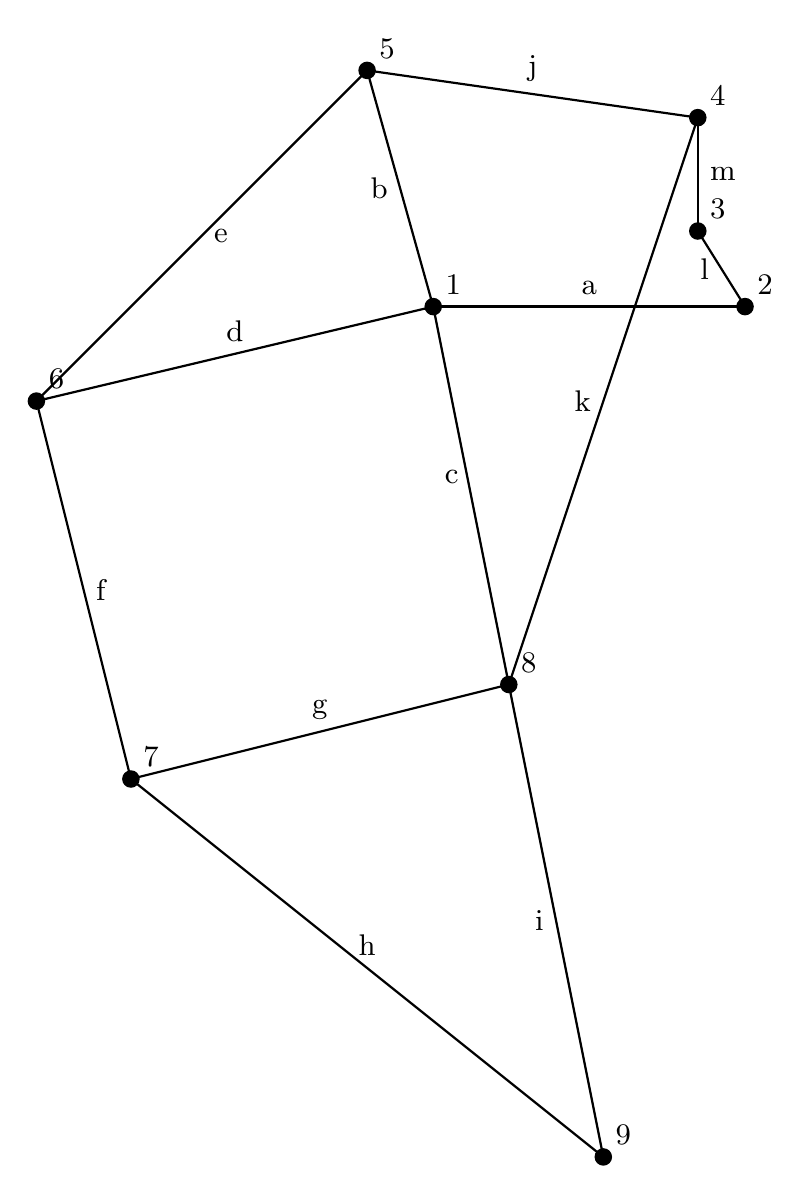
\begin{tikzpicture}[scale=0.12, thick, every node/.style={scale=1.2}]

  \coordinate (P1) at (22,30);
  \coordinate (P2) at (55,30);
  \coordinate (P3) at (50,38);
  \coordinate (P4) at (50,50);
  \coordinate (P5) at (15,55);
  \coordinate (P6) at (-20,20);
  \coordinate (P7) at (-10,-20);
  \coordinate (P8) at (30,-10);
  \coordinate (P9) at (40,-60);

  \draw (P1) -- (P2) node[midway,above] {\small a};
  \draw (P2) -- (P3) node[midway,left] {\small l};
  \draw (P3) -- (P4) node[midway,right] {\small m};
  \draw (P4) -- (P5) node[midway,above] {\small j};
  \draw (P5) -- (P1) node[midway,left] {\small b};
  \draw (P5) -- (P6) node[midway,right] {\small e};
  \draw (P6) -- (P1) node[midway,above] {\small d};
  \draw (P6) -- (P7) node[midway,right] {\small f};
  \draw (P1) -- (P8) node[midway,above left] {\small c};
  \draw (P7) -- (P8) node[midway,above] {\small g};
  \draw (P7) -- (P9) node[midway,above] {\small h};
  \draw (P9) -- (P8) node[midway,left] {\small i};
  \draw (P8) -- (P4) node[midway,left] {\small k};
  
  \foreach \p/\n in {P1/1, P2/2, P3/3, P4/4, P5/5, P6/6, P7/7, P8/8, P9/9}
  \filldraw (\p) circle (23pt) node[above right] {\small \n};  
  \end{tikzpicture}
  \end{figure}

  Estos números sagrados son la base del diseño de las patas del mecanismo y se utilizan para calcular las longitudes y ángulos necesarios para que el mecanismo funcione correctamente.

  De acuerdo a estos se establece el factor de escala del mecanismo, que es la relación entre las dimensiones del mecanismo y las dimensiones reales de las patas. Este factor de escala se utiliza para ajustar el tamaño del mecanismo a las necesidades específicas del proyecto y garantizar que funcione correctamente.

  Como medida base se toma la longitud \textbf{a} que pretende ser de 38 cm pero se escalará a 20 cm de acuerdo a la siguiente expresión:
  \begin{equation}
    \text{Factor de escala} = \frac{\text{Longitud deseada}}{\text{Longitud original}} = \frac{20}{38} \approx 0.5263
  \end{equation}

